\section{Анимация}
\label{sec:animation}

Анимация на экране компьютера использует ту же технику что и мультипликационные 
фильмы. Большая часть изображения не меняется, только подвижная часть изменяет 
цвет своих пикселей. При работе с анимацией, сразу же возникает проблема 
скорости рисования. Она зависит от сложности вычислений и производительности 
процессора. Поэтому, чтобы анимация была переносима и имела одинаковый эффект, 
необходимо учитывать производительность процессора. Чтобы получить плавную 
анимацию, желательно вывести на экран на новое положение анимационный объект, 
затем стереть старый, учитывая при этом пересечение областей обоих объектов.

\subsubsection{Перемещение объекта}

Для упрощения задачи, мы будем перемещать объекты простой формы, как 
прямоугольник. Остаётся проблема заполнения экрана за перемещённым объектом.

Мы хотим перемещать прямоугольник в замкнутом пространстве. Объект перемещается 
с определённой скоростью в направлении X и Y. Если он дойдёт до границы 
графического окна, объект отскочит он него на определённый угол отражения. 
Объект перемещается из одного положения в другое без перекрывания между новой и 
старой позицией. В зависимости от текущего положения \code{(x, y)}, размера 
объекта \code{(sx, sy)} и его скорости \code{(dx, dy)} функция \code{calc\_pv} 
вычисляет, учитывая границы окна, новое положение и новую скорость.

\begin{lstlisting}[language=OCaml]
# let calc_pv (x,y) (sx,sy) (dx,dy) = 
   let nx1 = x+dx     and  ny1 = y + dy
   and nx2 = x+sx+dx  and  ny2 = y+sy+dy
   and ndx = ref dx   and  ndy = ref dy 
   in  
     ( if (nx1 < 0) || (nx2 >= Graphics.size_x()) then ndx := -dx ) ;
     ( if (ny1 < 0) || (ny2 >= Graphics.size_y()) then ndy := -dy ) ;
     ((x+ !ndx, y+ !ndy), (!ndx, !ndy)) ;;
val calc_pv :
  int * int -> int * int -> int * int -> (int * int) * (int * int) = <fun>
\end{lstlisting}

Функция перемещая прямоугольник, указанный положением \code{pos} и размером 
\code{size}, \code{n} раз, полученная траектория учитывает скорость 
\code{speed} и границы окна. Путь перемещения, изображённый на рисунок 
\ref{??}, получен инверсией растрового изображения, который соответствует 
перемещённому прямоугольнику.

\begin{lstlisting}[language=OCaml]
# let  roule_fond pos taille vit n =
   let (x, y) = pos and (sx,sy) = taille in
   let mem = ref (Graphics.get_image x y sx sy) in 
   let rec roule_aux  x y vit n =
    if n = 0 then Graphics.moveto x y
    else 
     let ((nx,ny),n_vit) = calc_pv (x,y) (sx,sy) vit 
     and old_mem = !mem in 
      mem := Graphics.get_image nx ny sx sy ;
      Graphics.set_color Graphics.blue;
      Graphics.fill_rect nx ny sx sy;
      Graphics.draw_image (inv_image old_mem) x y;
      roule_aux nx ny n_vit (n-1)
   in roule_aux x y vit n ;;
val roule_fond : int * int -> int * int -> int * int -> int -> unit = <fun>
\end{lstlisting}

Следующий код соответствует изображениям на рисунке \ref{??}, первое получено 
на красном фоне, второе --- перемещением объекта по картинке Jussieu.

\begin{lstlisting}[language=OCaml]
# let anim_rect () = 
   Graphics.moveto 105 120 ;
   Graphics.set_color Graphics.white;
   Graphics.draw_string "Début" ;
   roule_fond (140,120) (8,8) (8,4) 150 ;
   let (x,y) = Graphics.current_point() in 
    Graphics.moveto (x+13) y ;
   Graphics.set_color Graphics.white;
   Graphics.draw_string "Fin" ;;
val anim_rect : unit -> unit = <fun>
# anim_rect();;
- : unit = ()
\end{lstlisting}

\begin{figure}[h]
	\center{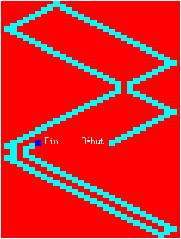
\includegraphics[scale=0.7]{drafts/book-ora015}
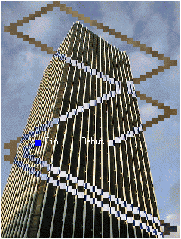
\includegraphics[scale=0.7]{drafts/book-ora016}}
	\caption{\label{fig:moving_an_object}Перемещение объекта}
\end{figure}

Наша задача была упрощена тем, что не было пересечений между новым и старым 
положением объекта. В противном случае, необходимо написать функцию вычисляющую 
это пересечение, что может быть более или менее сложно в зависимости от формы 
объекта. В настоящем примере с квадратом, при пересечении квадратов получается 
прямоугольник, который необходимо стереть.
